\documentclass{beamer}
% \documentclass[handout]{beamer}


% \usetheme{CambridgeUS}
\usetheme{Pittsburgh}
\usecolortheme{wolverine}
% \usetheme{Montpellier}
\usepackage{commands}
\usepackage{faktor}
\usepackage{xfrac} 

\newcommand{\isoclass}[1]{[#1]}
\newcommand{\wkclass}[1]{\{ #1 \}}

%AUTHOR DETAILS
%%%%%%%%%%%%%%%%%%%%%%%%%%%%%%%%%%%%%%%%%%%%%%%%
\title[]{Computing of abelian varieties over finite fields}
\author[Marseglia Stefano]{Marseglia Stefano}
\institute[]{Stockholm University}
\date{06 June 2018}

\begin{document}

\begin{frame}
\titlepage
\end{frame}

\begin{frame}{\ }
\begin{center}
\Large
   PAPER I : Computing the ideal class monoid of an order
\end{center}
\end{frame}

\begin{frame}{background in number theory}
\begin{itemize}
   \pause \item A \textbf{number field} is a finite field extension of $\Q$.\\
	 eg. \[\Q(\alpha) = \Q[x]/(f) \text{ where } f=x^3+10x^2-8,\]
   \pause \item An \textbf{order} is a subring of a finite product of number fields that has maximal $\Z$-rank.\\
   \pause eg.
	    \begin{align*}
	      R & =\Z[\alpha] = \Z \oplus \alpha \Z \oplus \alpha^2 \Z, \\
	      S & = \Z \oplus \alpha \Z \oplus \frac{\alpha^2}{2} \Z, \\
	      \cO & = \Z \oplus \frac{\alpha}{2} \Z \oplus \frac{\alpha^2}{4} \Z
	    \end{align*}
\end{itemize}
\end{frame}

\begin{frame}{background in number theory}
\begin{itemize}
   \item A \textbf{fractional $R$-ideal} $I$ is a finitely generated sub-$R$-module of $K$ such that $I\otimes \Q=K$\\
	\pause  eg. \begin{align*}
		& I = 3\Z\oplus (\alpha+2)\Z \oplus (\alpha^2+2)\Z, \\
	        & J = 3\Z\oplus (\alpha+2)\Z \oplus \left(\frac{\alpha^2+2\alpha}{8}\right)\Z,\\
	        & \text{also $R, S$ and $\cO$ are frac. $R$-ideals.}
	     \end{align*}
    \pause \item Two fractional $R$-ideals $I$ and $J$ are \textbf{isomorphic}
	 \[ I\simeq_R J \Longleftrightarrow \exists x \in K^\times \text{ s.t.~} xI=J \]
	 eg. \[ (\alpha^2+\alpha)J = I , \qquad I = (-17+18\alpha+2\alpha^2)R. \]
\end{itemize}
\end{frame}

\begin{frame}{ICM: ideal class monoid}
\begin{itemize}
\item Define the \textbf{ideal class monoid} of $R$ as
\[\ICM(R) := \faktor{\set{\text{fractional $R$-ideals}}}{\simeq_R}\]
     \pause  eg. \[ \ICM(R) = \set{ \isoclass{R},\isoclass{S},\isoclass{\cO},\textcolor{red}{\isoclass{S^t}}}, \]
	 where 
	  \[ \red{S^t}=\Z\oplus \left(\frac{2+F}{4}\right)\Z\oplus \left(\frac{188 -312 F + F^2}{3784} \right)\Z \]
\end{itemize}
\end{frame}

\begin{frame}{ICM: ideal class monoid}
 \begin{itemize}
   \item A fractional $R$-ideal $I$ is called \textbf{invertible} if there exists an $R$-ideal $J$ such that 
   \[ IJ = R. \]
   \pause \item Put
   \vspace{-1 em}\[ \Pic(R) := \dfrac{\set{\parbox{8 em}{\center\vspace{-0.5 em} invertible\\ fractional $R$-ideals}}}{\simeq_R} \qquad \textcolor{blue}{\parbox{7 em}{it can be computed efficiently}}\]
   \pause \item We have
   \[ \ICM(R) \supseteq \Pic(R) \hspace{2.5 cm} \textcolor{blue}{\text{with equality iff $R=\cO_K$}} \]
   \pause \item ...and actually
   \[ \ICM(R) \supseteq \bigsqcup_{\scriptsize\parbox{5 em}{$R\subseteq S \subseteq \cO_K$\\over-orders}}\Pic(S) \qquad \textcolor{blue}{\text{with equality iff $R$ is Bass}} \]
\end{itemize}
\end{frame}

\begin{frame}{simplify the problem}
   Study the isomorphism problem locally: (Dade, Taussky, Zassenhaus '62)\\
\pause  \textbf{weak equivalence}:
\[I_\p\simeq_{R_\p} J_\p \text{ for every }\p\in \mSpec(R)\]
\pause \vspace{-6mm}\[\Updownarrow\]
\[1\in (I:J)(J:I)\quad \textcolor{blue}{\text{easy to check!}}\]
\pause Let $\cW(R)$ be the set of weak eq.~classes...\\
\pause ...whose representatives can be found in
	\[\set{\text{sub-$R$-modules of $\faktor{\cO_K}{\frf_R}$}}\quad \textcolor{blue}{\parbox{10 em}{finite! and most of the time not-too-big ...}}\]
\end{frame}

\begin{frame}{Compute $\ICM(R)$ }
\pause Partition w.r.t.~the multiplicator rings:
    \begin{columns}
    \begin{column}{0.5\textwidth}
      \[ \cW(R) = \bigsqcup_{R\subseteq S \subseteq \cO_K} \overline \cW(S)\]
      \[\ICM(R) = \bigsqcup_{R\subseteq S \subseteq \cO_K} \overline \ICM(S)\]
    \end{column}
\pause
    \begin{column}{0.5\textwidth}  %%<--- here
	\begin{center}
	\textcolor{blue}{\parbox{10em}{the ``bar'' means ``only classes with multiplicator ring S''}} 
	\end{center}
    \end{column}
    \end{columns}
\pause
   \begin{theorem}[M.]
    For every over-order $S$ of $R$, $\Pic(S)$ acts freely on $\overline{\ICM(S)}$ and
    \[ \overline\cW(S) = \overline{\ICM(S)}/\Pic(S) \]
\pause Repeat for every $R\subseteq S \subseteq \cO_K$:
    \[ \rightsquigarrow \ICM(R).\]
   \end{theorem}
\end{frame}

\begin{frame}{Example 1}
\begin{figure}
    \begin{columns}%
        \begin{column}{0.6\textwidth}%
            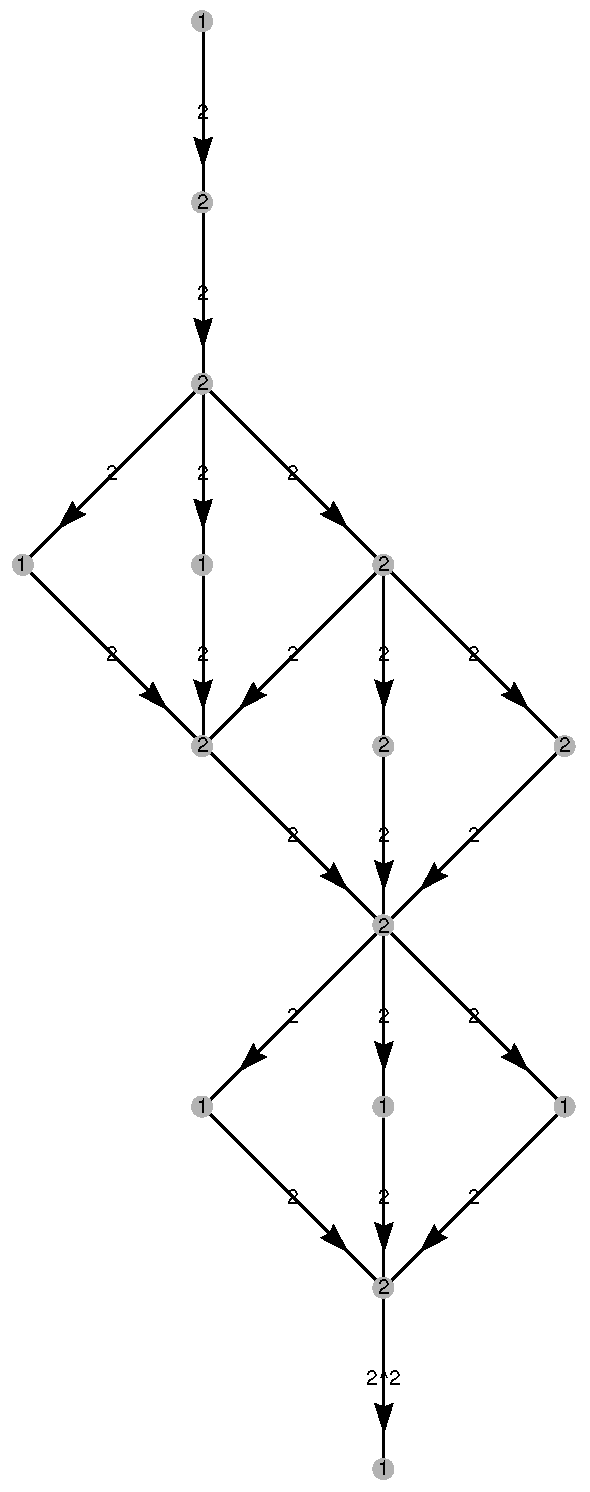
\includegraphics[width=0.5\textwidth]{graph-4}
        \end{column}%
        \begin{column}{0.4\textwidth}%
            Weak equivalence classes of the monogenic order of $\Q[x]/(f)$ where $f=x^3+31x^2+43x+77$.\\
	    - vertices are orders, labeled by $\# \bWk$\\
	    - edges are inclusions, labeled by the index
        \end{column}%
    \end{columns}
\end{figure}
\end{frame}

\begin{frame}{Example 2}
\vspace{-2 em}
\begin{figure}
    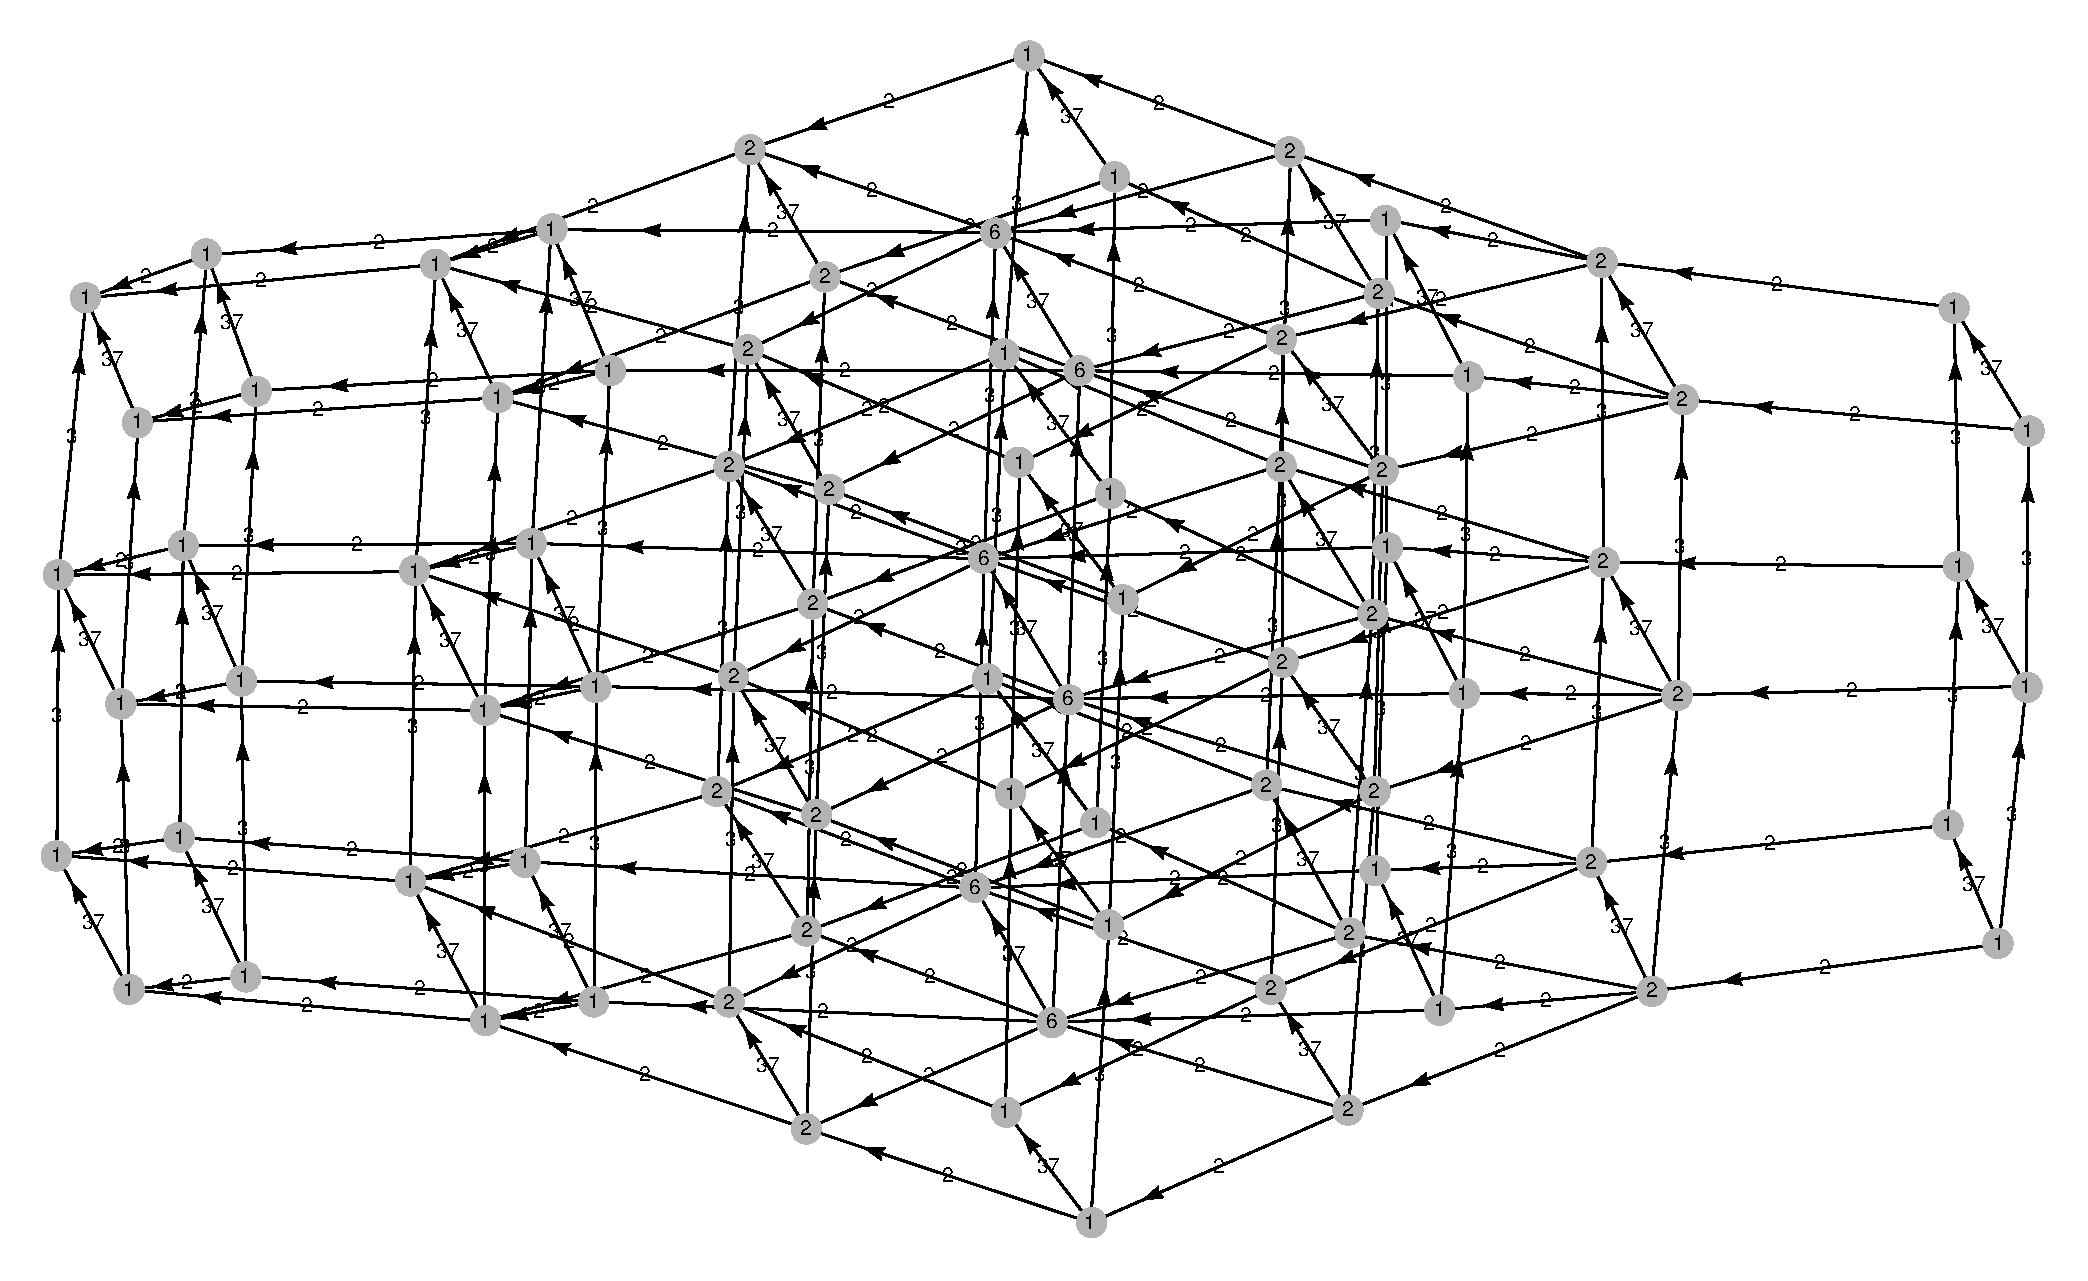
\includegraphics[width=1\textwidth]{graph-1}
\end{figure}
\vspace{-2 em} Weak equivalence classes of the monogenic order of $\Q[x]/(f)$ where
\[ f=(x^2+4x+7)(x^3−9x^2−3x−1). \] 
\end{frame}

\begin{frame}{\ }
\begin{center}
\Large
   PAPER II : Computing square-free polarized abelian varieties over finite fields
\end{center}
\end{frame}

\begin{frame}{square-free abelian varieties}
Fix a \textbf{ordinary square-free} characteristic $q$-Weil polynomial $h$.\\
\[\rightsquigarrow \text{an isogeny class $\cC_h$ (by Honda-Tate)}.\]
Put 
\[K := \Q[x]/(h) \text{ and } F:= x \mod h. \]
\pause
% \vspace{-2 em}
\begin{theorem}[M.]
\[\begin{array}{cc}
\faktor{\set{\text{Ordinary abelian varieties over $\F_q$ in $\cC_h$}}}{\simeq} & \\
\updownarrow & \\
\faktor{\set{ \text{fractional ideals of $\Z[F,q/F] \subset K$ } }}{\simeq} & =:\textcolor{blue}{\ICM(\Z[F,q/F])}\\ 
  & \textcolor{blue}{\text{ ideal class monoid} }
  \end{array}\]
\end{theorem}
\pause \vspace{-1.2 em} Also \textbf{polarizations} can be described in terms of fractional ideals!

\end{frame}


\begin{frame}{Example}
\begin{itemize}
 \item Let $h(x)=x^8 - 5x^7 + 13x^6 - 25x^5 + 44x^4 - 75x^3 + 117x^2 - 135x + 81$;
 \item $\rightsquigarrow$ isogeny class of an simple ordinary abelian varieties over $\F_{3}$ of dimension $4$;
 \item Let $F$ be a root of $h(x)$ and put $R:=\Z[F,3/F]\subset \Q(F)$;
 \item $8$ over-orders of $R$: two of them are not Gorenstein;
 \item $\#\ICM(R) = 18 \rightsquigarrow 18$ isom.~classes of AV in the isogeny class;
 \item $5$ are not invertible in their multiplicator ring;
 \item $8$ classes admit principal polarizations;
 \item $10$ isomorphism classes of princ. polarized AV.
\end{itemize}
\end{frame}
\begin{frame}{Example}
Concretely:
{\scriptsize \begin{align*}
  \begin{split} 
  I_1 = & 2645633792595191 \Z \oplus (F + 836920075614551) \Z \oplus (F^2 + 1474295643839839)\Z \oplus\\
	& \oplus (F^3 + 1372829830503387)\Z \oplus (F^4 + 1072904687510)\Z \oplus\\
	& \oplus \frac{1}{3}(F^5 + F^4 + F^3 + 2F^2 + 2F + 6704806986143610)\Z \oplus\\
	& \oplus \frac{1}{9}(F^6 + F^5 + F^4 + 8F^3 + 2F^2 + 2991665243621169) \Z \oplus\\
	& \oplus \frac{1}{27}(F^7 + F^6 + F^5 + 17F^4 + 20F^3 + 9F^2 + 68015312518722201)\Z\\
  \end{split}
\intertext{principal polarizations:}
  \begin{split}
  x_{1,1} = \frac{1}{27}( & -121922F^7 + 588604F^6 - 1422437F^5 +\\
			  & +1464239F^4 + 1196576F^3 - 7570722F^2 + 15316479F - 12821193)\\ 
%   \end{split}\\
%   \begin{split}
  x_{1,2} = \frac{1}{27}( & 3015467F^7 - 17689816F^6 + 35965592F^5 -\\
			  & -64660346F^4 + 121230619F^3 - 191117052F^2 + 315021546F - 300025458)\\
  \end{split}\\
  & \End(I_1) =  R\\
  & \#\Aut(I_1,x_{1,1}) = \#\Aut(I_1,x_{1,2}) = 2
 \end{align*}}
\end{frame}


\begin{frame}{Example}
 
{\scriptsize \begin{align*}
  \begin{split} 
  I_7 = & 2\Z\oplus(F + 1)\Z\oplus(F^2 + 1)\Z\oplus(F^3 + 1)\Z\oplus(F^4 + 1)\Z\oplus\frac13(F^5 + F^4 + F^3 + 2F^2 + 2F + 3)\Z \oplus \\ 		      & \oplus\frac{1}{36}(F^6 + F^5 + 10F^4 + 26F^3 + 2F^2 + 27F + 45)\Z\oplus\\
	& \oplus \frac{1}{216}(F^7 + 4F^6 + 49F^5 + 200F^4 + 116F^3 + 105F^2 + 198F + 351)\Z\\
  \end{split}
\intertext{principal polarization:}\\[-7ex]
  \begin{split}
  x_{7,1} = \frac{1}{54}(20F^7 - 43F^6 + 155F^5 - 308F^4 + 580F^3 - 1116F^2 + 2205F - 1809)
  \end{split}\\
  \begin{split}
  \End(I_7) & = \Z \oplus  F\Z \oplus  F^2\Z \oplus  F^3\Z \oplus  F^4\Z \oplus
  \frac{1}{3}(F^5 + F^4 + F^3 + 2F^2 + 2F)\Z \oplus \\
	& \oplus \frac{1}{18}(F^6 + F^5 + 10F^4 + 8F^3 + 2F^2 + 9F + 9)\Z \oplus\\
	& \oplus \frac{1}{108}(F^7 + 4F^6 + 13F^5 + 56F^4 + 80F^3 + 33F^2 + 18F + 27)\Z\\
  \end{split}\\
  & \#\Aut(I_7,x_{7,1}) = 2
\end{align*}}             
$I_1$ is invertible in $R$, but $I_7$ is not invertible in $\End(I_7)$.
\end{frame}

\begin{frame}{some results from computations}
  \begin{tabular}{| c | c | c | c | c |}
  \hline
		& isogeny cl.     & isom. cl.     & \parbox{3.5 em}{isom.~cl.\\non pol.} & princ. pol.\\\hline
     $\F_2,g=2$ & $14/34$         & $21$	  & $7$ 	       & $15$ \\\hline
     $\F_2,g=3$ & $81/210$        & $225$	  & $107$ 	       & $141$ \\\hline
     $\F_3,g=2$ & $35/62$         & $75$	  & $23$ 	       & $58$ \\\hline
     $\F_3,g=3$ & $315/670$ (wip) & $2329$  	  & $1244$	       & $1325$ \\\hline
     $\F_5,g=2$ & $94/128$        & $457$	  & $207$ 	       & $286$ \\\hline
     $\F_5,g=3$ & $213/2994$ (wip)& $11733$	  & $9336$ 	       & $2721$ \\\hline
     $\F_7,g=2$ & $167/207$       & $1322$  	  & $638$ 	       & $793$ \\\hline
     $\F_7,g=3$ & $176/7968$ (wip)& $10379$  	  & $8026$ 	       & $2702$ \\\hline
     $\F_{11},g=2$ & $352/400$    & $4925$  	  & $2675$ 	       & $2797$ \\\hline
     $\F_{11},g=3$ & $188/30530$ (wip)    & $18513$ & $14291$	       & $4830$ \\\hline
  \end{tabular}
  
  (wip) = work in progress
\end{frame}

\begin{frame}{other results}
  \pause PAPER II:
    \begin{itemize}
       \item Period matrices of the canonical lift to $\C$ for square-free ordinary abelian varieties.
       \pause \item Isomorphism classes of square-free abelian varieties over $\F_p$ (away from $\sqrt{p}$) using Centeleghe/Stix (2015).
    \end{itemize}
  \pause PAPER III:
    \begin{itemize}
        \item Isomorphism classes of ab. var. with char. poly of the form $h^r$ (with Bass assumption).
       \pause \item Polarizations are work in progress.
    \end{itemize}
  \pause PAPER IV:
    \begin{itemize}
       \item Use the results from PAPER II and PAPER III to distinguish which isomorphism classes are extension of the base field.
    \end{itemize}  
    
\end{frame}

\begin{frame}{}
\begin{center}
{\Large Thank you!}
\end{center}
\end{frame}

\end{document}
